\documentclass{article}
\usepackage{arxiv}
\usepackage[utf8]{inputenc}
\usepackage[T1]{fontenc}
\usepackage[none]{hyphenat}      % no automatic hyphens at line breaks
\usepackage{hyperref}
\usepackage{url}
\usepackage{booktabs}
\usepackage{amsfonts,amsmath}
\usepackage{microtype}
\usepackage{graphicx}
\usepackage{xcolor}
\usepackage{natbib}
\usepackage{caption}
\usepackage{enumitem}
\setlist{nosep,leftmargin=*}
\setlength{\emergencystretch}{2em}
\hypersetup{colorlinks=true,linkcolor=black,citecolor=black,urlcolor=blue!60!black}
\renewcommand{\headeright}{}
\renewcommand{\undertitle}{Project report}
\renewcommand{\shorttitle}{NYU Tandon Deep Learning F26, Project 1}
\date{November 2026}

\title{An SE-ResNet-26 Under 5M Parameters for CIFAR-10}

\author{
  Uvindu Salgado \\ uis202 \\ \texttt{uis202@nyu.edu}
  \And
  Michael Wang \\ mzw2010 \\ \texttt{mzw2010@nyu.edu}
}

\begin{document}
\maketitle

\begin{center}
\textbf{Kaggle team:} Punters \quad$\cdot$\quad
\textbf{Code:} \url{https://github.com/breeze215/cifar10-resnet-5m}
\end{center}

\begin{abstract}
We design and train a residual network with at most 5 million parameters for the course's CIFAR-10 Kaggle challenge.
Our final model is an SE-ResNet-26 with 4,810,754 trainable parameters, trained from scratch. It reaches 97.9\%
accuracy on our held out validation images, 89.7\% on the public leaderboard and \textbf{88.3\%} on the private
leaderboard, which placed our team \textbf{11th}, 23 places above our public rank. We report all thirteen of our
training runs, including the ones that did not work. Stronger data augmentation gave the largest improvement, 3.0
points on the public leaderboard. After that, training on more data, sharpness aware minimization, knowledge
distillation, a deeper network and robustness oriented augmentation all scored between 89.0\% and 89.8\% on the public
leaderboard, even when they clearly improved validation accuracy. We think two things explain this. The test images
look different from the training images (brighter, higher in contrast and more often grayscale), and a score computed
on 1,000 images has a standard error of about one point, which is larger than most of the differences between our
models. We therefore chose our final submissions by validation accuracy, and they turned out to be our two best
submissions on the private leaderboard.
\end{abstract}

\section{Overview}

The task is to classify the $32\times32$ color images of CIFAR-10 \citep{krizhevsky2009cifar} with a convolutional
network that has residual connections, at most 5 million trainable parameters, no pretrained weights and no outside
data. We train on the 50,000 labeled training images. Kaggle scores submissions on 2,000 hidden test images, split into
a public half that is visible during the competition and a private half that decides the final ranking.

\paragraph{Summary of findings.}
\begin{itemize}
  \item \textbf{Final model.} An SE-ResNet-26: three stages of 5, 4 and 3 residual blocks at 64, 128 and 256 channels,
  each block ending in a squeeze and excitation gate \citep{hu2018se}, for 4,810,754 parameters. It is trained for 600
  epochs with TrivialAugment \citep{muller2021trivialaugment}, CutMix \citep{yun2019cutmix}, label smoothing and an average
  of the weights over training. It scores 97.90\% on validation, 89.7\% public and 88.3\% private.
  \item \textbf{Biggest improvement.} Moving from simple crop, flip and Cutout augmentation to TrivialAugment, CutMix and
  weight averaging, together with a deeper network, raised our public score from 86.9\% to 89.9\%.
  \item \textbf{Changes that did not show up on the leaderboard.} Training on all 50,000 images, SAM \citep{foret2021sam},
  AugMix \citep{hendrycks2020augmix}, distillation \citep{hinton2015distilling}, the deeper SE network (0.5 points better on
  validation) and augmentation aimed at robustness (0.6 points better on shifted validation images) all scored between
  89.0\% and 89.8\% public.
  \item \textbf{Why we think this happened.} The hidden test images are distributed differently from the training images
  (Section~\ref{sec:shift}), and the public score is too noisy to separate models that differ by less than about a point
  (Section~\ref{sec:noise}).
  \item \textbf{How we picked our submissions.} Since the public score could not tell our models apart, we chose our two
  final submissions based on validation accuracy and robustness. They became our two best submissions on the private
  leaderboard (88.3\% and 88.0\%), while v2, our best public score at 89.9\%, came seventh of our ten submissions there.
\end{itemize}

\section{Methodology}

\subsection{Evaluation protocol}
We set aside 5,000 of the 50,000 training images, chosen with random seed 0, and use the same 5,000 images for every
validation number in this report. We never train on them. Validation accuracy uses the averaged weights described in
Section~\ref{sec:recipe} and averages the predictions on each image and its mirror image. To make a submission we retrain
the same settings on all 50,000 images. These runs have no validation images left, so for them we report the validation
accuracy of the matching run trained on 45,000 images. Test predictions average ten versions of each test image: the
image and its mirror, each also shifted by 2 pixels up, down, left and right. All training ran on NVIDIA T4 GPUs on
Kaggle, in mixed precision \citep{micikevicius2018mixed} with PyTorch \citep{paszke2019pytorch}, usually two runs at a time.

\subsection{Architecture}
\label{sec:arch}
Each residual block computes $y = \mathrm{ReLU}(S(x) + F(x))$. Here $F$ is a $3{\times}3$ convolution, batch normalization
(BN) and a ReLU, followed by a second $3{\times}3$ convolution and BN \citep{he2016resnet,ioffe2015bn}. $S$ is the identity,
or a $1{\times}1$ convolution with BN when the number of channels or the resolution changes. As in most CIFAR ResNets
(for example \citealp{kuangliu2017pytorchcifar}), the first layer is a single $3{\times}3$ convolution with stride 1 and no
max pooling, so the network starts at the full $32\times32$ resolution.

\paragraph{Choosing depth and width.} The usual ResNet-18 layout ends with a stage at 512 channels, but a single block at
that width already costs 3.67M parameters, most of our budget. We therefore use three stages, at $32\times32$,
$16\times16$ and $8\times8$, and spend the parameters on depth. Table~\ref{tab:arch} lists the three networks we trained.
v1 used a few wide blocks. v2 used more, narrower blocks, the same layout a previous project in this course arrived at
\citep{thakur2023efficient}. The final network adds a fifth block to the first stage and a squeeze and excitation (SE)
gate to every block. An SE gate rescales each channel using that channel's average over the whole image. All the SE
gates together cost only 39,608 parameters (0.8\% of the model). Putting the extra block in the second stage instead
would have taken us to 5,033,282 parameters, over the limit.

\begin{table}[h]
\centering\small
\caption{The three networks we trained, plus the large teacher we considered but never trained (Section~\ref{sec:kd}).
Layers counts the convolutions on the main path plus the final linear layer, the way ResNet-18 is counted. MACs is the
number of multiply and add operations needed for one image.}
\label{tab:arch}
\begin{tabular}{lccccc}
\toprule
Model & Channels per stage & Blocks per stage & Layers & Parameters & MACs \\
\midrule
v1: ResNet-14 & 80, 160, 320 & 2, 2, 2 & 14 & 4,337,370 & 658M \\
v2: ResNet-24 & 64, 128, 256 & 4, 4, 3 & 24 & 4,697,162 & 799M \\
\textbf{Final: SE-ResNet-26} & 64, 128, 256 & 5, 4, 3 with SE & 26 & \textbf{4,810,754} & 874M \\
\midrule
\textit{Teacher: WRN-28-10} & 160, 320, 640 & 4, 4, 4 & 28 & 36,479,194 & 5,243M \\
\bottomrule
\end{tabular}
\end{table}

\subsection{Training recipe}
\label{sec:recipe}
Every run uses SGD with Nesterov momentum 0.9 \citep{sutskever2013momentum}, batch size 128, and weight decay of
$5\times10^{-4}$ on the convolution and linear weights. The learning rate rises linearly to 0.1 over the first five epochs,
then follows a cosine curve down to zero \citep{loshchilov2017sgdr}. We use label smoothing of 0.1 \citep{szegedy2016inception}.
v1 used standard augmentation: random crops after padding each side by 4 pixels, horizontal flips and Cutout
\citep{devries2017cutout}. From v2 on, each training image also receives one random operation from TrivialAugment (for
example a change in brightness, contrast, color or sharpness, or a small rotation), is turned grayscale with probability
0.05, and half of the batches use CutMix, which pastes a patch of one image into another and mixes their labels in the
same proportion. We also keep an exponential moving average (EMA) of the weights with decay 0.9995
\citep{polyak1992averaging} and use it for all evaluation. The final model trains for 600 epochs, about 32 seconds per
epoch on one T4.

\subsection{The experiments}
Table~\ref{tab:runs} lists all thirteen runs in the order we ran them, by both of us. Most come in pairs: one run trained on
45,000 images to measure validation accuracy, and one trained on all 50,000 images to submit. Each experiment was chosen
based on what the earlier ones showed us, and Section~\ref{sec:wrong} goes through the ones that did not work out.

\begin{table}[h]
\centering\footnotesize
\setlength{\tabcolsep}{3.5pt}
\caption{All thirteen training runs, in order. All scores are in percent. Val is accuracy on our 5,000 held out images. Public and Private are the
Kaggle scores on the two halves of the hidden test set (1,000 images each). A blank Val means the run used all 50,000
images, so nothing was left to validate on; a blank Public and Private means the run was used only for validation and
never submitted. Bold rows are our two final submissions.}
\label{tab:runs}
\begin{tabular}{rllcrccc}
\toprule
\# & Run & What changed & Images & Epochs & Val & Public & Private \\
\midrule
1 & v1 & ResNet-14; crop, flip, Cutout, label smoothing & 45k & 200 & 96.66 & 86.9 & 85.3 \\
2 & v2 & ResNet-24; TrivialAugment, grayscale, CutMix, EMA & 45k & 300 & 97.40 & 89.9 & 86.5 \\
3 & v2, all data & run 2 settings on all images & 50k & 300 & & 89.0 & 87.0 \\
4 & SAM & run 2 trained with SAM ($\rho = 0.05$) & 45k & 200 & 97.22 & 89.3 & 86.8 \\
5 & AugMix & run 2 with AugMix, not TrivialAugment & 45k & 300 & 97.20 & 89.4 & 86.0 \\
6 & no grayscale & run 3 without the grayscale step & 50k & 300 & & 89.8 & 86.9 \\
7 & distillation & ResNet-24 student; teachers: runs 2 and 4 & 45k & 200 & 97.34 & & \\
8 & distillation & same; teachers: runs 2, 3 and 4 & 50k & 200 & & 89.0 & 87.5 \\
9 & v4 & SE-ResNet-26, 600 epochs & 45k & 600 & 97.90 & & \\
\textbf{10} & \textbf{v4 (\texttt{final})} & \textbf{run 9 settings on all images} & \textbf{50k} & \textbf{600} & & \textbf{89.7} & \textbf{88.3} \\
11 & robust & run 9 with AugMix, color jitter, blur & 45k & 600 & 97.82 & & \\
\textbf{12} & \textbf{robust (\texttt{final\textasciicircum2})} & \textbf{run 11 settings on all images} & \textbf{50k} & \textbf{600} & & \textbf{89.6} & \textbf{88.0} \\
13 & fine tuning & run 9 trained further on hard views & 45k & 200 & 97.44 & 88.9 & 85.7 \\
\bottomrule
\end{tabular}
\end{table}

\section{Experiments That Did Not Pan Out}
\label{sec:wrong}

\subsection{Better validation accuracy stopped helping on the leaderboard}
\label{sec:shift}
Going from v1 to v2 added 0.74 points of validation accuracy and 3.0 points on the public leaderboard. Going from v2 to
v4 added another 0.50 points of validation accuracy, yet the public score went down by 0.2 points (Figure~\ref{fig:valpub}).
Our test accuracy (88 to 90\%) is about 8 points below our validation accuracy (97 to 98\%). A gap that large means the
test images are very unlikely to come from the same distribution as the training images.

To see how they differ, we compared simple pixel statistics of the training images and the test images
(Table~\ref{tab:shift}). The test images are brighter, higher in contrast and sharper, and three times as likely to be
grayscale. This looks like a test set that was collected separately from the original data, as with CIFAR-10.1
\citep{recht2018cifar,recht2019imagenet}. On such test sets, models typically lose several points of accuracy, but better
models still tend to score higher \citep{miller2021line}. That would explain both of our observations. The augmentation
added in v2 (TrivialAugment's brightness, contrast, color and sharpness changes, plus grayscale) covers the directions
in which the test images differ, which produced the large gain. Once those were covered, extra validation accuracy carried
over to the test set only weakly.

\begin{figure}[h]
\centering
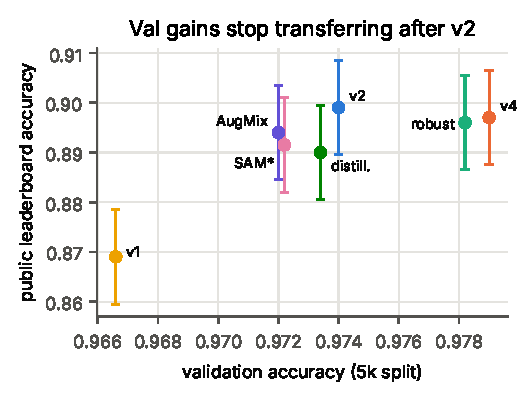
\includegraphics[width=\linewidth]{../figures/fig_val_vs_public.pdf}
\caption{Validation accuracy against the public (left) and private (right) leaderboard score of each submission. Runs
trained on all 50,000 images use the validation accuracy of the matching 45,000 image run. Error bars are plus or minus one
standard error of a score on 1,000 images (0.95 points).}
\label{fig:valpub}
\end{figure}

\begin{table}[h]
\centering\small
\caption{How the hidden test images differ from the training images. We computed these from the test images' pixels
alone; we never had the test labels.}
\label{tab:shift}
\begin{tabular}{lccc}
\toprule
Statistic & Training images & Test images & Test / training \\
\midrule
Mean brightness & 0.473 & 0.491 & 1.04 \\
Contrast (standard deviation within an image) & 0.211 & 0.220 & 1.04 \\
Edge strength (mean difference between neighboring pixels) & 0.054 & 0.059 & 1.08 \\
Share of grayscale images & 1.1\% & 3.3\% & 2.9 \\
\bottomrule
\end{tabular}
\end{table}

\paragraph{A note on the grayscale setting.} We looked at the test images only through the averages in
Table~\ref{tab:shift}. We never had their labels and never trained on them, so v2 and our final models are valid
submissions. One setting was influenced by this analysis, though: we added the grayscale step (probability 0.05) after
seeing that the test set has more grayscale images. Choosing training settings from test set statistics comes close to
what the rules call model selection on the evaluation set, so we checked whether it mattered. Run 6 is v2 trained on all
50,000 images without the grayscale step. It scored 89.8\% public and 86.9\% private, against 89.0\% and 87.0\% for
run 3, which is the same run with the step included. The setting made no measurable difference. Our robust recipe
(Section~\ref{sec:robust}) was motivated by the general finding that the test set looks different, but it uses standard
augmentations at their usual strengths.

\subsection{We mistook noise for real differences}
\label{sec:noise}
After v2, we trained the same settings on all 50,000 images (run 3) and a version with SAM (run 4). Both scored lower on
the public leaderboard (89.0\% and 89.3\%, against 89.9\%), and at first we concluded that both changes had hurt. That was
the wrong conclusion, and the reason is the size of the public test set.

A score measured on 1,000 images carries an uncertainty of about one point: if a model's true accuracy is 90\%, its score
on 1,000 random images has a standard error of $\sqrt{0.9 \times 0.1 / 1000} \approx 0.95$ points. Comparing two models is
a bit more precise, because they get most of the same images right. For a typical pair of our submissions, the two models
give different answers on 6.2\% of the test images, about 62 of the 1,000 public images. Both models score the same on the
other 938 images, so only those 62 decide which model comes out ahead. If the two models are equally good, each of those
62 images is as likely to favor one model as the other, like a coin toss. Over 62 tosses, the difference in correct answers
typically varies by about $\sqrt{62} \approx 8$ images, which is 0.8 points. The spread of our public scores after v2,
89.0\% to 89.9\%, is about what we would expect from models of equal quality.

The private leaderboard confirms this. The two halves of the test set ranked our submissions quite differently: run 3,
which looked worse than v2 on the public half, scored higher on the private half (87.0\% against 86.5\%), and v2, our best
public score, came seventh out of our ten submissions. Our team moved from 34th place on the public leaderboard to 11th
on the private one. From v2 onward we compared models by validation accuracy and by the robustness scorecard in
Section~\ref{sec:robust}, and used the public score only as a sanity check.

\subsection{SAM: an unequal comparison}
SAM reached 97.22\% after 200 epochs, compared with 97.40\% for v2 after 300 epochs. SAM computes two gradients per step,
so we gave it fewer epochs to keep the training time about the same. That makes the comparison unfair, since SAM may
simply have needed the longer schedule. With a fixed GPU allowance of 30 hours per week on Kaggle we did not rerun it, so
this result does not tell us whether SAM helps on this problem.

\subsection{Distillation from our own models}
\label{sec:kd}
The rules allow distillation as long as the teacher is trained from scratch on the allowed data, so we distilled our own
models into a ResNet-24 student, with temperature 2, a weight of 0.9 on the distillation loss, and the teacher and student
seeing the same augmented batch \citep{beyer2022patient}. On validation the student (97.34\%) did not beat its best teacher
(v2, 97.40\%). The reason is that the ensemble of v2 and the SAM model scored only 97.52\%, just 0.12 points above v2: two
models with the same architecture and augmentation make largely the same mistakes, so together they give the student
little new information. When we paired v2 with the AugMix model instead, which was trained differently, the ensemble rose
to 97.68\% (0.28 points above v2), which suggests that diversity is what matters. Our teachers were also trained with label
smoothing, which is known to make worse teachers \citep{muller2019labelsmoothing}. On the private half, the distilled
submission was our third best (87.5\%), so distillation may have helped a little on the test set; with one run we cannot
tell.

We also considered a much larger teacher. Only the final model is limited to 5M parameters, so we implemented a WRN-28-10
\citep{zagoruyko2016wrn} with 36.5M parameters, with a check that refuses to write predictions for any model over 5M. We
dropped it before training once v4 reached 97.90\%. The published result for a WRN-28-10 trained with TrivialAugment is
about 97.5\% \citep{muller2021trivialaugment}, so it was unlikely to beat our student, and training it would have used
about half of our remaining GPU time.

\subsection{Robustness gains in the wrong directions}
\label{sec:robust}
Because the leaderboard could not measure small improvements, we built a robustness scorecard: validation accuracy on
seven shifted copies of our own validation images, inspired by CIFAR-10-C \citep{hendrycks2019corruptions}. The shifts are
15\% brighter, 25\% more contrast, sharpening, blur, grayscale, JPEG compression at quality 60 and Gaussian noise. The
model never sees JPEG compression or noise during training. Our robust recipe replaced TrivialAugment with a random
choice between TrivialAugment and AugMix, and added color jitter, grayscale and blur to some images. We moved the color
jitter to the GPU because AugMix made the CPU data loading too slow to keep up. The robust recipe raised mean shifted
accuracy from 94.27\% to 94.87\% (2.3 points on JPEG, which it never trained on, and 1.8 points on blur) while keeping
clean accuracy (Figure~\ref{fig:score}). It did not raise the leaderboard score: 89.6\% public and 88.0\% private, against
89.7\% and 88.3\% for v4. The scorecard shows why. On the shifts where the test set actually differs (brightness,
contrast, sharpening and grayscale), v4 and the robust model are within 0.2 points of each other. Our earlier AugMix run
(run 5) showed the same pattern: on a separate benchmark of seven corruptions it scored 3.2 points higher than v2, but it
reached only 89.4\% public and 86.0\% private.

\begin{figure}[h]
\centering
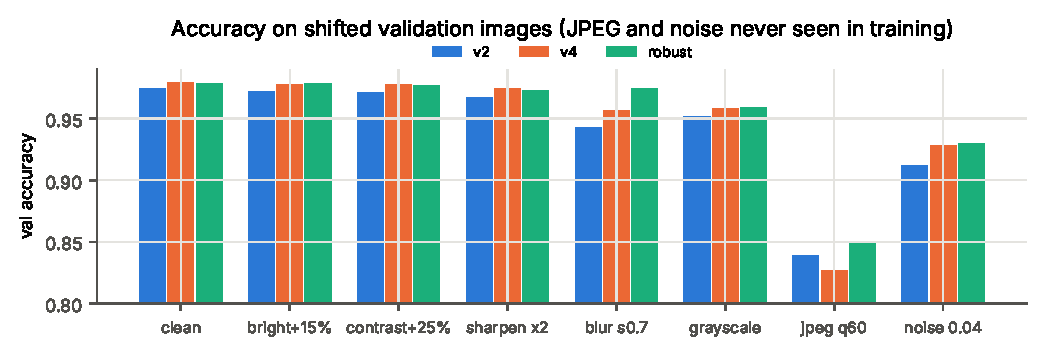
\includegraphics[width=\linewidth]{../figures/fig_scorecard.pdf}
\caption{Robustness scorecard on shifted copies of our 5,000 validation images. The robust recipe gains the most on blur
and JPEG, which do not resemble the test images. On brightness, contrast, sharpening and grayscale it is level with v4.}
\label{fig:score}
\end{figure}

\subsection{Fine tuning a finished model}
Our last experiment continued training the v4 validation model for 200 more epochs. In two thirds of each batch, each image
was replaced by the harder of two random photometric versions of it, an idea inspired by AugMax \citep{wang2021augmax}.
Restarting the learning rate at 0.018 dropped validation accuracy from 97.90\% to 84.3\% within two epochs, and it only
recovered to 97.44\% (97.48\% with ten view test predictions, against 97.86\% before). We think raising the learning rate
again pushed the weights away from the good solution the original training had settled into, and 200 epochs were not
enough to get back. This run was also our second lowest private score (85.7\%).

\subsection{Engineering mistakes}
\begin{itemize}
  \item \textbf{A false alarm from float32 arithmetic.} Our first comparison of training and test statistics gave a
  training set mean of 0.328 in every channel, far from CIFAR-10's usual 0.49, 0.48 and 0.45, which made it look as if the
  training images had been darkened. The real cause was rounding error from adding up $1.5\times10^8$ values in float32.
  In float64 the values came out as expected, and since then we compute all statistics, including the normalization
  constants, in float64.
  \item \textbf{A race condition.} When we ran two jobs in one session, both processes wrote the same image cache file at
  the same time. We caught this in a local test before it cost any GPU time and fixed it by having each process write to
  its own temporary file and then rename it.
  \item \textbf{Naming.} Our code calls v2 ``ResNet-26''; by the standard convention it has 24 layers, and the final model 26.
\end{itemize}

\section{Results}

\paragraph{Final model.} The SE-ResNet-26 in Table~\ref{tab:arch} starts with a $3{\times}3$ convolution with 64 channels.
Stage 1 has five blocks at 64 channels and $32\times32$, stage 2 has four blocks at 128 channels and $16\times16$, and
stage 3 has three blocks at 256 channels and $8\times8$. Every block ends in an SE gate, and the network finishes with
global average pooling and a linear layer from 256 features to 10 classes. It has \textbf{4,810,754 trainable parameters}:
68.7\% in stage 3, 23.4\% in stage 2, 7.8\% in stage 1, and 39,608 (0.8\%) in the SE gates. We submitted two versions,
both trained on all 50,000 images for 600 epochs: \texttt{final} (v4 recipe) and \texttt{final\textasciicircum2} (robust
recipe). Kaggle ranks a team by the better of its two selected submissions, so our final score is 88.3\%, 11th place.

\begin{table}[h]
\centering\small
\caption{Final results. Validation numbers come from the run trained on 45,000 images with the same settings as each
submission.}
\label{tab:final}
\begin{tabular}{lcccccc}
\toprule
Submission & Parameters & Val & Val (10 views) & Shifted val & Public & Private \\
\midrule
\texttt{final} (v4) & 4,810,754 & 97.90\% & 97.86\% & 94.27\% & 89.7\% & \textbf{88.3\%} \\
\texttt{final\textasciicircum2} (robust) & 4,810,754 & 97.82\% & 97.92\% & 94.87\% & 89.6\% & 88.0\% \\
v2 (best public score) & 4,697,162 & 97.40\% & 97.54\% & 93.65\% & 89.9\% & 86.5\% \\
\bottomrule
\end{tabular}
\end{table}

Figure~\ref{fig:curves} shows the training curves. With strong augmentation, validation accuracy keeps rising as the
learning rate decays: the last 20\% of training still adds 1.2 to 1.4 points (v4 goes from 96.6\% to 97.9\%, v2 from
96.0\% to 97.4\%), which suggests longer schedules help. v1, with weak augmentation, overfits the most: 99.45\% training
accuracy against 96.66\% on validation.

\begin{figure}[!htb]
\centering
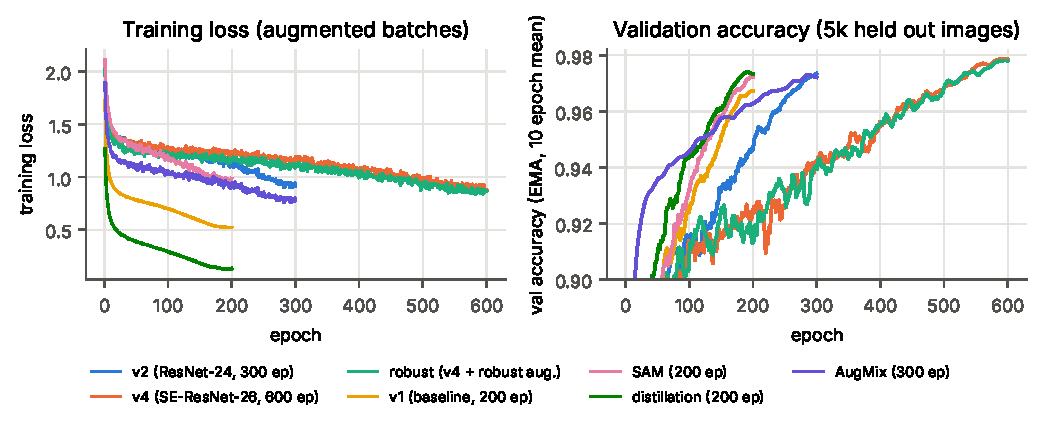
\includegraphics[width=\linewidth]{../figures/fig_curves.pdf}
\caption{Training loss and validation accuracy for every run with a validation set. The loss values are not comparable
across runs, because CutMix, label smoothing and distillation change the training targets.}
\label{fig:curves}
\end{figure}

\paragraph{Reproducibility.} The repository contains the exact script and the executed Kaggle notebook for every run, the
weights of both submissions and their validation runs, and \texttt{results.ipynb}. That notebook prints the parameter
counts, recomputes validation accuracy from the saved weights (it reproduces the logged 97.40\%, 97.90\% and 97.82\% for v2,
v4 and robust exactly), and regenerates both submission files, which match the uploaded files on 2,000 of 2,000 test
images for \texttt{final} and 1,999 of 2,000 for \texttt{final\textasciicircum2}.

\section{Lessons and limitations}
\begin{itemize}
  \item \textbf{Find out how noisy the leaderboard is before trusting it.} After v2, almost every change we made moved the
  public score by less than its uncertainty, and we read two of those moves as regressions. Working out the standard error
  and how often our models disagree would have told us much earlier to rely on validation accuracy instead.
  \item \textbf{Validation and test accuracy can diverge when the test set is shifted.} Augmentation that matched the
  shift helped a lot; general robustness and extra validation accuracy helped much less.
  \item \textbf{Ensembles and distillation need different models.} Teachers trained the same way added almost nothing.
  \item \textbf{Compare methods with the same training budget.} Our SAM comparison was muddied by its shorter schedule.
  \item \textbf{Limitations.} We trained each configuration only once, so we do not know how much the results vary
  between random seeds. With 5,000 validation images, differences smaller than about 0.2 points (one standard error) are
  not meaningful. In v2 we changed the network and the augmentation at the same time, so we cannot separate their effects.
\end{itemize}

\paragraph{Contributions.} Both authors contributed equally to this project. Uvindu focused on the training pipeline, the
SE network and the distillation and robustness experiments. Michael focused on the AugMix experiment and its corruption
benchmark, the grayscale ablation, and the comparison of teacher ensembles for distillation.

\paragraph{Acknowledgements.} Our residual block, CIFAR style first layer and baseline optimizer settings (SGD with learning
rate 0.1, momentum 0.9, weight decay $5\times10^{-4}$, a cosine schedule, and crop and flip augmentation) follow the
conventions of \citet{kuangliu2017pytorchcifar}. All code in our repository was written by us.

\bibliographystyle{plainnat}
\bibliography{references}

\end{document}
